\section{Evaluation}\label{sec:eval}

We evaluate \sysname{} using a combination of testbed experiments and numerical
experiments. Our evaluation focuses on three key questions: $(i)$ Can \sysname{}
prevent deadlock? $(ii)$ Is \sysname{} scalable for large data center networks?,
and $(iii)$ Does \sysname{} have a performance penalty?

\begin{figure}
	\centering
	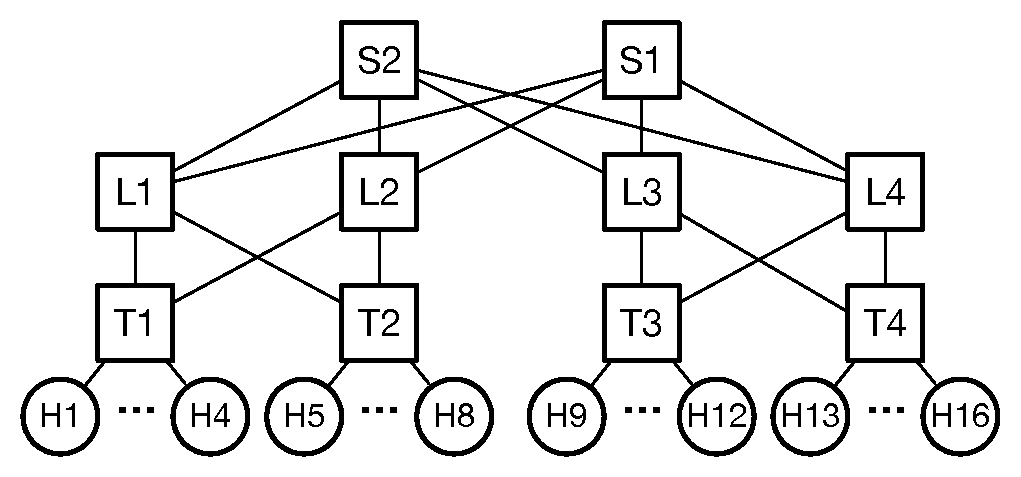
\includegraphics[width=0.45\textwidth] {figs/testbed_topo}
	\caption{Testbed Topology.}\label{fig:testbed_topo}
\end{figure}

\textbf{Testbed setup}: We use a small Clos network as our testbed with 16
servers and 10 switches, as shown in Figure~\ref{fig:testbed_topo}. Each server
is a Dell PowerEdge R730 server with a 40GbE Mellanox ConnectX-3 Pro NIC, two
16-core Intel E5-2698 2.3GHz CPUs, 256GB memory and 2TB hard disk. Each switch
is a Arista 7060CX-32S switch with 32 100GbE ports and 16MB packet buffer. Our
switches support PFC with at most 8 priority classes. Our ConnectX-3 Pro NICs
support RoCEv2 and DCQCN protocol.

\subsection{Deadlock prevention}\label{subsec:exp_validation}

\begin{figure}[t]
	%\vspace{-0.1in}
	\centering
	
	\subfloat[short for lof][Without \sysname] {
		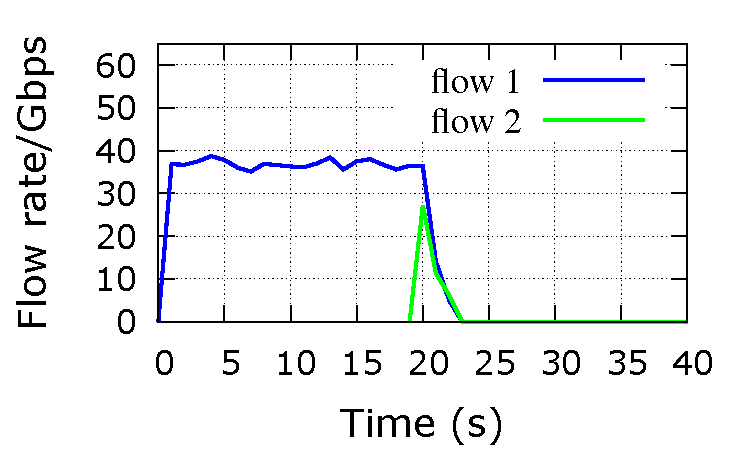
\includegraphics[width=0.25\textwidth] {figs/validation_nonloopcase_flowrate_notagger}
	}
	\subfloat[short for lof][With \sysname]{
		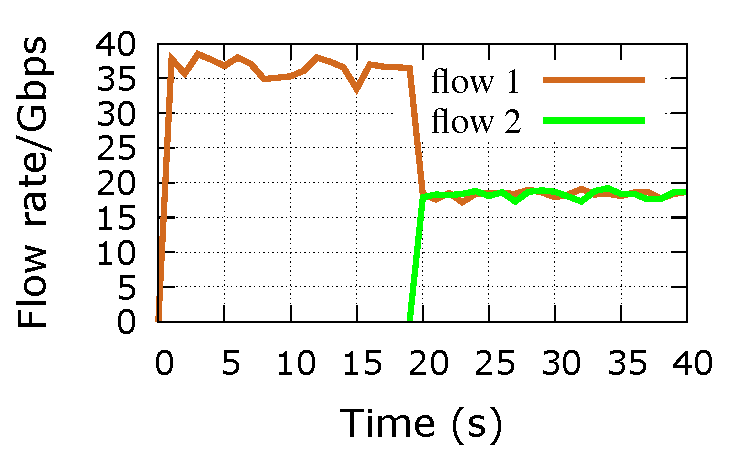
\includegraphics[width=0.25\textwidth] {figs/validation_nonloopcase_flowrate_tagger}
	}
	
	\caption{Clos deadlock due to 1-bounce paths}\label{fig:exp_validation_nonloop}
	
\end{figure}

\begin{figure}[t]
	%\vspace{-0.1in}
	\centering
	
	\subfloat[short for lof][Scenario] {
		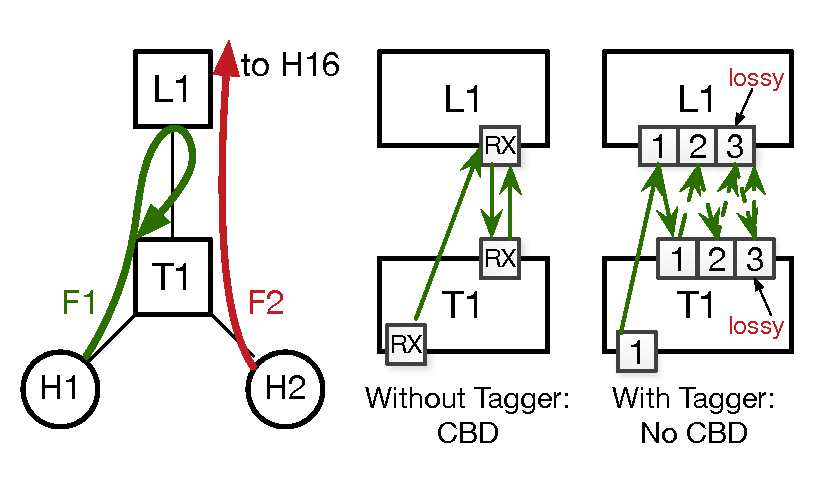
\includegraphics[width=0.26\textwidth] {figs/validation_loopcase_scenario}
	}
	\subfloat[short for lof][Rate of flow 2]{
		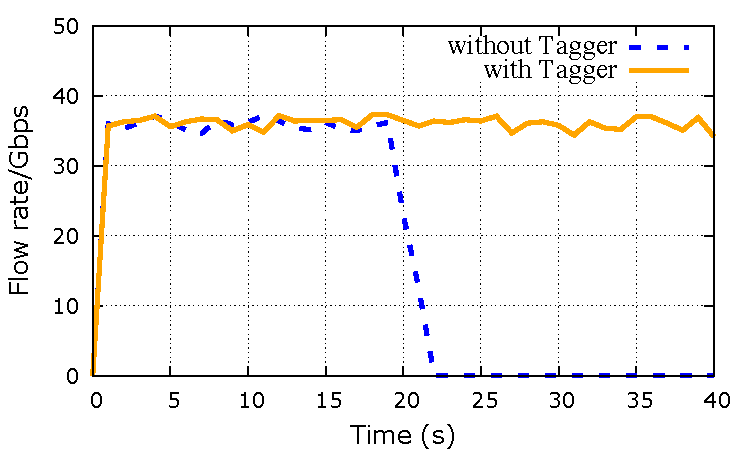
\includegraphics[width=0.24\textwidth] {figs/validation_loopcase_flowrate}
	}
	
	\caption{Deadlock due to routing loop}\label{fig:exp_validation_loop}
	
\end{figure}

\begin{figure}[t]
	%\vspace{-0.1in}
	\centering
	
	\subfloat[short for lof][4-to-1 shuffle with \sysname] {
		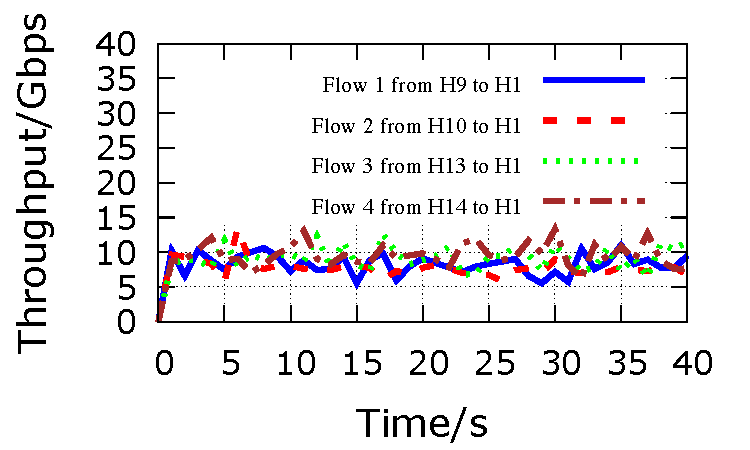
\includegraphics[width=0.25\textwidth] {figs/validation_pp_manytoone_tagger}
	}
	\subfloat[short for lof][4-to-1 shuffle without \sysname]{
		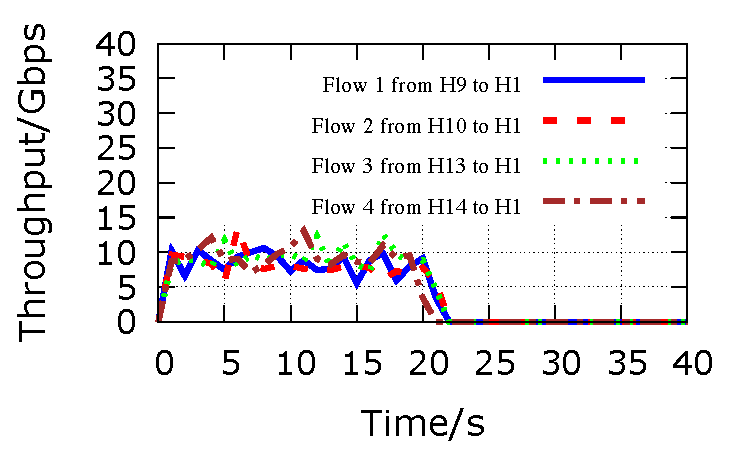
\includegraphics[width=0.25\textwidth] {figs/validation_pp_manytoone_notagger}
	}

	\subfloat[short for lof][1-to-4 shuffle with \sysname] {
	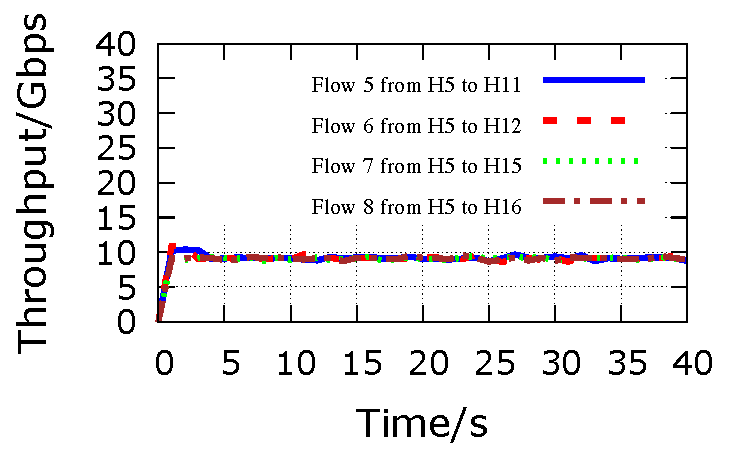
\includegraphics[width=0.25\textwidth] {figs/validation_pp_onetomany_tagger}
}
\subfloat[short for lof][1-to-4 shuffle without \sysname]{
	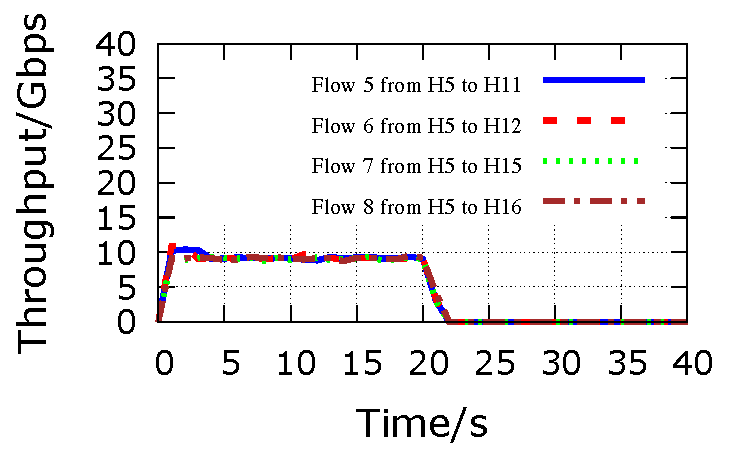
\includegraphics[width=0.25\textwidth] {figs/validation_pp_onetomany_notagger}
}
	
	\caption{PFC PAUSE propagation due to deadlock (\textcolor{red}{This is expected results. Will be updated later.}) }\label{fig:exp_validation_propagation}
	
\end{figure}


We have already {\em proved} that \sysname{} prevents deadlock, so the
experiments in this section are primarily illustrative.

\textbf{Deadlock due to one bounce:} We recreate the scenario shown in
Figure~\ref{fig:clos_1_bounce}, where 1-bounce paths lead to CBD.  In this
experiment, we start the green flow at time 0, and the blue flow at time 20.
Figure~\ref{fig:exp_validation_nonloop} shows the rate of the two flows with and
without \sysname{}.  Without \sysname{}, deadlock occurs and rate of both flows
are reduced to 0. With \sysname{}, and ELR set to include shortest paths and
1-bounce paths, there is no deadlock and flow rates are not affected.

\textbf{Deadlock due to routing loop:} As shown in
Figure~\ref{fig:exp_validation_loop}(a), we generate 2 flows across different
ToRs, i.e.,  $F_1$ from H1 to H15 and $F_2$ from H2 to H16. At time = 20s, we
install a bad route at L1 to let $F_1$ enter a routing loop between T1 and L1.
The path taken by $F_2$ also traverses link T1-L1.  ELR is set to include the
shortest paths and 1-bounce paths.

In Figure~\ref{fig:exp_validation_loop}(b), we plot the rate of $F_2$ with and
without \sysname{}. As we can see, if \sysname{} is not used, deadlock occurs
and $F_2$ is paused due to propagation of PFC PAUSE. With \sysname{}, there is
no deadlock and rate of $F_2$ is not affected by the routing loop. Note that
throughput of $F_1$ is zero, as packets are dropped due to TTL expiration.

The key takeaway here is that \sysname{} was able to successfully deal with a
routing loop.

\textbf{PAUSE propagation due to deadlock:} Once deadlock occurs, PFC PAUSE will propagate and may finally pause all the flow running in the datacenter network. In this experiment, we run a many-to-one data shuffle from H9, H10, H13 and H14 to H1, and a one-to-many data shuffle from H5 to  H11, H12, H15 and H16 simultaneously.  We emulate the CBD scenario where the flow from H9 to H1 and the flow from H5 to H15 enter two 1-bounce paths due to link failures. 

In Figure~\ref{fig:exp_validation_propagation}, we plot the throughput of all 8 flows with and without \sysname{}. Without \sysname{}, all flows get paused due to PFC PAUSE propagation and throughput is reduced to zero. With \sysname{}, flows are not affected by link failures.


\subsection{Scalability}
\label{subsec:exp_overhead}

As discussed in \S\ref{sec:challenges}, commodity switches can support only a
limited number of lossless queues.  We have already shown that on a Clos
topology, \sysname{} requires $k+1$ lossless priorities to support paths with
up to $k$ bounces. In this section, we consider other topologies.

\begin{table}[t]
	\centering
	\scalebox{0.85}{
		\begin{tabular}{|r|r|r|r|r|}
			\hline
			Switch $\#$ &  \multicolumn{1}{c|}{\tabincell{c}{\text{Switch} \\ \text{port $\#$}}}   &  \multicolumn{1}{c|}{\tabincell{c}{\text{Network} \\ \text{diameter}}}  &	 \multicolumn{1}{c|}{\tabincell{c}{\text{$\#$ of lossless} \\ \text{priority classes}}}   &
			\multicolumn{1}{c|}{\tabincell{c}{Max \text{$\#$ of rules} \\
				\text{at a switch}}}\\
			\hline
			\hline
			10 & 12 & 5 & 2 & 10 \\
			\hline
			100 & 32 & 6 & 3 &  37 \\
			\hline
			500 & 64 & 6 & 3 & 76 \\
			\hline
			1,000 & 64 & 6 & 3 & 88 \\
			\hline
			2,000 & 64 & 7 & 3 & 98 \\
			\hline
			
		\end{tabular}
	}
	\caption{Jellyfish with shortest paths.}
	\label{table:jellyfish_shortestpath}
\end{table}

Jellyfish topology is an r-regular random graph, characterized by the the number
of switches (N), the number of ports a switch has (k) and the number of ports
used to connect with other switches (r) (the remaining $k-r$ ports are for
servers). In our experiment, we let r = k/2.  We construct the routing paths by
building destination-rooted shortest-path spanning trees at all the servers.

Table~\ref{table:jellyfish_shortestpath}, shows the number of lossless priority
classes needed for a variety of network sizes. We see that \sysname{} requires
only three classes even for a network with 2000 switches.

The table also shows the maximum number of rules needed at a switch for various
configurations~\footnote{Different switches require different number of rules
due to the random nature of the topology.}. Even with 2000 switches, we need
just 98 ACLs at a switch. Modern commodity switches can support 1-4K ACLs.

\begin{table}[t]
	\centering
	\scalebox{0.85}{
		\begin{tabular}{|r|r|r|r|r|}
			\hline
			Switch $\#$ &  \multicolumn{1}{c|}{\tabincell{c}{\text{Switch} \\ \text{port $\#$}}}   &  \multicolumn{1}{c|}{\tabincell{c}{\text{Network} \\ \text{diameter}}}  &	 \multicolumn{1}{c|}{\tabincell{c}{\text{$\#$ of lossless} \\ \text{priority classes}}}   &
			\multicolumn{1}{c|}{\tabincell{c}{Max \text{$\#$ of rules} \\
					\text{at a switch}}}\\
			\hline
			\hline
			10 & 12 & 5 & 3 & 23 \\
			\hline
			100 & 32 & 6 & 4 &  69 \\
			\hline
			500 & 64 & 6 & 4 &  107\\
			\hline
			1,000 & 64 & to be added & to be added & to be added \\
			\hline
			2,000 & 64 & to be added & to be added &  to be added\\
			\hline
			
		\end{tabular}
	}
	\caption{Jellyfish with shortest paths and random paths.}
	\label{table:jellyfish_randompath}
\end{table}


In Table~\ref{table:jellyfish_randompath}, we further create $N*10$ random paths in addition to the shortest paths.

\begin{table}[t]
	\centering
	\scalebox{0.85}{
		\begin{tabular}{|r|r|r|r|}
			\hline
			m    &	\multicolumn{1}{c|}{\tabincell{c}{\text{Network} \\ \text{diameter}}}&  \multicolumn{1}{c|}{\tabincell{c}{\text{$\#$ of lossless} \\ \text{priority classes}}}   &
			\multicolumn{1}{c|}{\tabincell{c}{Max \text{$\#$ of rules} \\
					\text{at a switch}}}\\
			\hline
			\hline
			1 & 5 & 2 & 30 \\
			\hline
			2  & 5 & 2&  36 \\
			\hline
			4  & 5 & 2 &  41\\
			\hline
			8  & 5 & 2 & 44 \\
			\hline
			16  & 5& 3 &  47\\
			\hline
			
		\end{tabular}
	}
	\caption{Jellyfish with m shortest paths between each server pair (under the settting of	switch number = 50, switch port number = 32).}
	\label{table:jellyfish_mshortestpath}
\end{table}


In Table~\ref{table:jellyfish_mshortestpath}, we  consider the case where there are m (m > 1) shortest paths between each server pair.


\begin{figure}
	\centering
	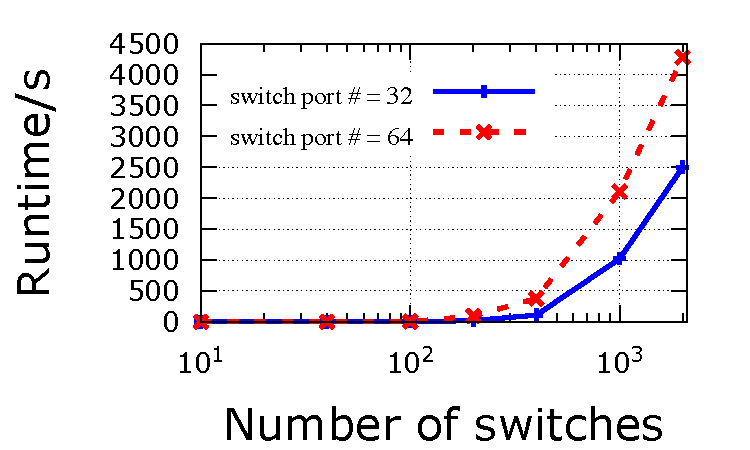
\includegraphics[width=0.45\textwidth] {figs/algo_runtime}
	\caption{Runtime of Algorithm~\ref{alg:greedy} on Jellyfish under different network scales ( one shortest path between each server pair).}
	\label{fig:algo_runtime}
\end{figure}

In Figure.~\ref{fig:algo_runtime}, we  plot the runtime of Algorithm~\ref{alg:greedy} on Jellyfish under different network scales.

\begin{table}[t]
	\centering
	\scalebox{0.87}{
		\begin{tabular}{|r|r|r|r|r|}
			\hline
			n  &  k &  \multicolumn{1}{c|}{\tabincell{c}{\text{Network} \\ \text{diameter}}}  &	\multicolumn{1}{c|}{\tabincell{c}{\text{$\#$ of lossless} \\ \text{priority classes}}}   &
			\multicolumn{1}{c|}{\tabincell{c}{Max \text{$\#$ of rules at} \\
					\text{a switch}}}\\
			\hline
			\hline
			4 & 1 & 4 & 2 & 12 \\
			\hline
			8 & 2 & 6 & 3 &  30\\
			\hline
			8 & 3 & 8 & 4 &  41\\
			\hline
			16 & 4 & 10 & 5 &  90\\
			\hline
			16 & 5 & 12 & 6 &  108\\
			\hline
			
		\end{tabular}
	}
	\caption{BCube with k shortest paths between every server pair.}
	\label{table:bcube_kpaths}
\end{table}

In Table~\ref{table:bcube_kpaths}, we consider $k$ shortest paths for BCube($n$,$k$), where $n$ is the number of switch ports and $k$ is the switch layers in the topology.

\begin{table}[t]
	\centering
	\scalebox{0.88}{
		\begin{tabular}{|r|r|r|r|r|}
			\hline
		k &  \multicolumn{1}{c|}{\tabincell{c}{\text{Network} \\ \text{diameter}}}    &	\multicolumn{1}{c|}{\tabincell{c}{\text{$\#$ of lossless} \\ \text{priority classes}}}   &
			\multicolumn{1}{c|}{\tabincell{c}{Max \text{$\#$ of rules at} \\
					\text{a switch}}}\\
			\hline
			\hline
			4 & 6 & 2 & 14 \\
			\hline
			8 & 6 & 2 &  24 \\
			\hline
			16 & 6 & 2 &  44 \\
			\hline
			32 & 6 & 2 &  84 \\
			\hline
			64 & 6 & 2 &  164 \\
			\hline
		\end{tabular}
	}
	\caption{F10 with shortest paths and 1-bounce paths.}
	\label{table:F10_onebounce}
\end{table}

In Table~\ref{table:F10_onebounce}, we consider all shortest paths and 1-bounce paths for F10($k$), where $k$ is the number of switch ports.

\subsection{Performance penalty}\label{subsec:exp_performanceoverhead}

\begin{figure}
	\centering
	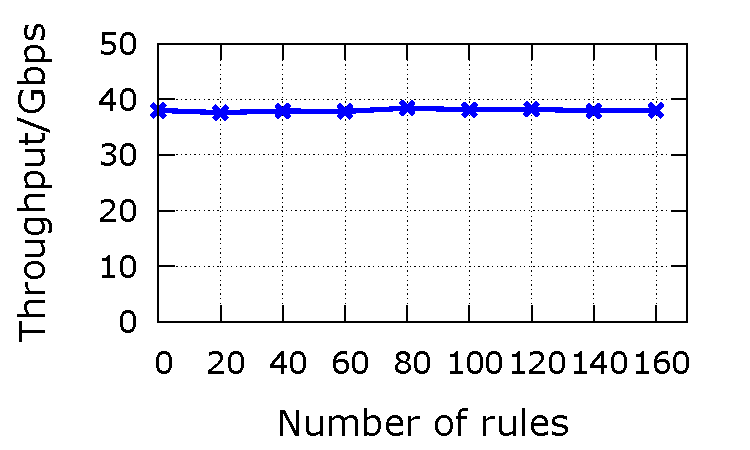
\includegraphics[width=0.4\textwidth] {figs/overhead_avgthrpt}
	\caption{RDMA Throughput with different number of rules.}\label{fig:thrpt_overhead}
\end{figure}

\begin{figure}
	\centering
	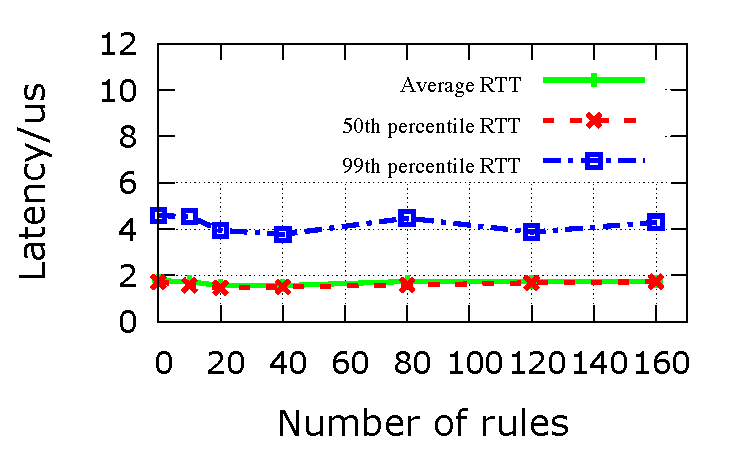
\includegraphics[width=0.45\textwidth] {figs/RDMAlatency_overhead}
	\caption{RDMA latency with different number of rules.}\label{fig:latency_overhead}
\end{figure}

At run time, the only impact of \sysname{} is that the packet has
to traverse the ACL rules. These are installed in TCAM, and hence induce
no discernible penalty, as illustrated next.

\textbf{Throughput penalty}: We generate one flow from H1 to H2, and observe
its average throughput over 100 seconds under varying number of \sysname{} rules
installed on T1. Figure~\ref{fig:thrpt_overhead} shows that the average
throughput is not affected.

\textbf{Latency penalty}: We install different number of \sysname{} rules in T1
and collect 5000 RTT samples between H1 and H2.
Table~\ref{fig:latency_overhead} shows that the number of installed rules does
not impact the latency of RDMA flows.

